% latex table generated in R 3.6.3 by xtable 1.8-4 package
% Thu Jan 18 11:46:06 2024
\begin{table}[ht]
\centering
\begin{tabular}{rlrrr}
  \hline
 & OTU & MeanRA & MedianRA & SE \\ 
  \hline
739141 & Methylobacterium sp. XJL & 0.00002928 & 0.00003017 & 0.00000178 \\ 
  419610 & Methylorubrum extorquens & 0.00005085 & 0.00005219 & 0.00000285 \\ 
  65958 & Komagataeibacter oboedien & 0.00004125 & 0.00004300 & 0.00000228 \\ 
  33995 & Komagataeibacter europaeu & 0.00003916 & 0.00003833 & 0.00000259 \\ 
  2558360 & Oecophyllibacter saccharovoran & 0.00005278 & 0.00005492 & 0.00000295 \\ 
  1389004 & Sulfitobacter sp. SK01 & 0.00005072 & 0.00004995 & 0.00000204 \\ 
  666509 & Planktomarina temperata & 0.00002576 & 0.00002657 & 0.00000178 \\ 
  2582913 & Luteithermobacter gelatinilyticu & 0.00006907 & 0.00006987 & 0.00000315 \\ 
  488446 & Burkholderia laten & 0.00003327 & 0.00003561 & 0.00000268 \\ 
  1855726 & Burkholderia sp. KK & 0.00009049 & 0.00009203 & 0.00000607 \\ 
  1795874 & Burkholderia sp. PAMC 2868 & 0.00003297 & 0.00003359 & 0.00000270 \\ 
  1385592 & Burkholderia mayoni & 0.00008178 & 0.00008543 & 0.00000760 \\ 
  977880 & Cupriavidus taiwanensis & 0.00002121 & 0.00001747 & 0.00000506 \\ 
  1537274 & Janthinobacterium sp. HH10 & 0.00003562 & 0.00003973 & 0.00000242 \\ 
  2808899 & Janthinobacterium lividu & 0.00002633 & 0.00002419 & 0.00000206 \\ 
  2823875 & Pseudomonas sp. Tri & 0.00003101 & 0.00003280 & 0.00000245 \\ 
  1573712 & Pseudomonas sp. R8 & 0.00002393 & 0.00002553 & 0.00000155 \\ 
  29442 & Pseudomonas tolaasi & 0.00004080 & 0.00004327 & 0.00000322 \\ 
  1301098 & Pseudomonas knackmussii & 0.00004764 & 0.00004121 & 0.00000580 \\ 
  237609 & Pseudomonas alkylphenolic & 0.00008176 & 0.00007784 & 0.00000497 \\ 
  1148509 & Pseudomonas proseki & 0.00004032 & 0.00004352 & 0.00000388 \\ 
  2505979 & Pseudomonas vicia & 0.00002989 & 0.00002956 & 0.00000272 \\ 
  47884 & Pseudomonas taetrolen & 0.00003525 & 0.00003477 & 0.00000196 \\ 
  158836 & Enterobacter hormaeche & 0.00005311 & 0.00005344 & 0.00000362 \\ 
  1134687 & Klebsiella michiganensi & 0.00003642 & 0.00004549 & 0.00000583 \\ 
  244366 & Klebsiella variicol & 0.00001960 & 0.00002579 & 0.00000441 \\ 
  83655 & Leclercia adecarboxylat & 0.00003913 & 0.00004189 & 0.00000243 \\ 
  2126321 & Nissabacter sp. SGAir020 & 0.00007781 & 0.00008511 & 0.00000553 \\ 
  55213 & Brenneria rubrifacien & 0.00001931 & 0.00001934 & 0.00000132 \\ 
  1052 & Halorhodospira halochlori & 0.00003505 & 0.00003734 & 0.00000250 \\ 
  2795687 & Thiohalobacter sp. COW & 0.00005266 & 0.00005382 & 0.00000260 \\ 
  2304594 & Marinobacter sp. Arc7-DN- & 0.00005741 & 0.00005295 & 0.00000278 \\ 
  2769486 & Marinobacter sp. LPB031 & 0.00005185 & 0.00005375 & 0.00000255 \\ 
  1420917 & Marinobacter salariu & 0.00005874 & 0.00006180 & 0.00000273 \\ 
  550540 & Ferrimonas balearica & 0.00006754 & 0.00006909 & 0.00000369 \\ 
  252514 & Microbulbifer thermotoleran & 0.00005079 & 0.00004900 & 0.00000309 \\ 
  670 & Vibrio parahaemolyticu & 0.00002349 & 0.00002564 & 0.00000185 \\ 
  2738883 & Candidatus Reidiella endopervernicos & 0.00004973 & 0.00004702 & 0.00000313 \\ 
  1725232 & Candidatus Desulfovibrio trichonympha & 0.00002010 & 0.00001904 & 0.00000233 \\ 
  67351 & Streptomyces californicu & 0.00006312 & 0.00005924 & 0.00000534 \\ 
  75293 & Streptomyces autolyticu & 0.00005799 & 0.00004972 & 0.00001076 \\ 
  33900 & Streptomyces murinu & 0.00004496 & 0.00004120 & 0.00000567 \\ 
  67260 & Streptomyces cinereorube & 0.00002862 & 0.00002962 & 0.00000202 \\ 
  1944646 & Phoenicibacter congonensi & 0.00001342 & 0.00001161 & 0.00000314 \\ 
  1126833 & Paenibacillus beijingensi & 0.00007217 & 0.00007351 & 0.00000286 \\ 
  79263 & Paenibacillus chitinolyticu & 0.00006405 & 0.00006215 & 0.00000237 \\ 
  2495582 & Paenibacillus albu & 0.00004750 & 0.00004437 & 0.00000211 \\ 
  43988 &   & 0.00002126 & 0.00002130 & 0.00000175 \\ 
  92942 & Nostoc lincki & 0.00002018 & 0.00001269 & 0.00000596 \\ 
  1306274 & Nostoc flagelliform & 0.00000908 & 0.00000664 & 0.00000159 \\ 
  289435 & Sphaerospermopsis kisselevian & 0.00001214 & 0.00001027 & 0.00000249 \\ 
  2527976 & Gimesia fumarol & 0.00004131 & 0.00004476 & 0.00000339 \\ 
  1851148 & Limihaloglobus sulfuriphilu & 0.00003138 & 0.00003198 & 0.00000276 \\ 
  51589 & Haloarcula hispanic & 0.00000693 & 0.00000692 & 0.00000056 \\ 
  1604004 & Halanaeroarchaeum sulfurireducen & 0.00003387 & 0.00003628 & 0.00000257 \\ 
   \hline
\end{tabular}
\caption{Keystone OTUs of } 
\end{table}
\begin{figure}
\centering
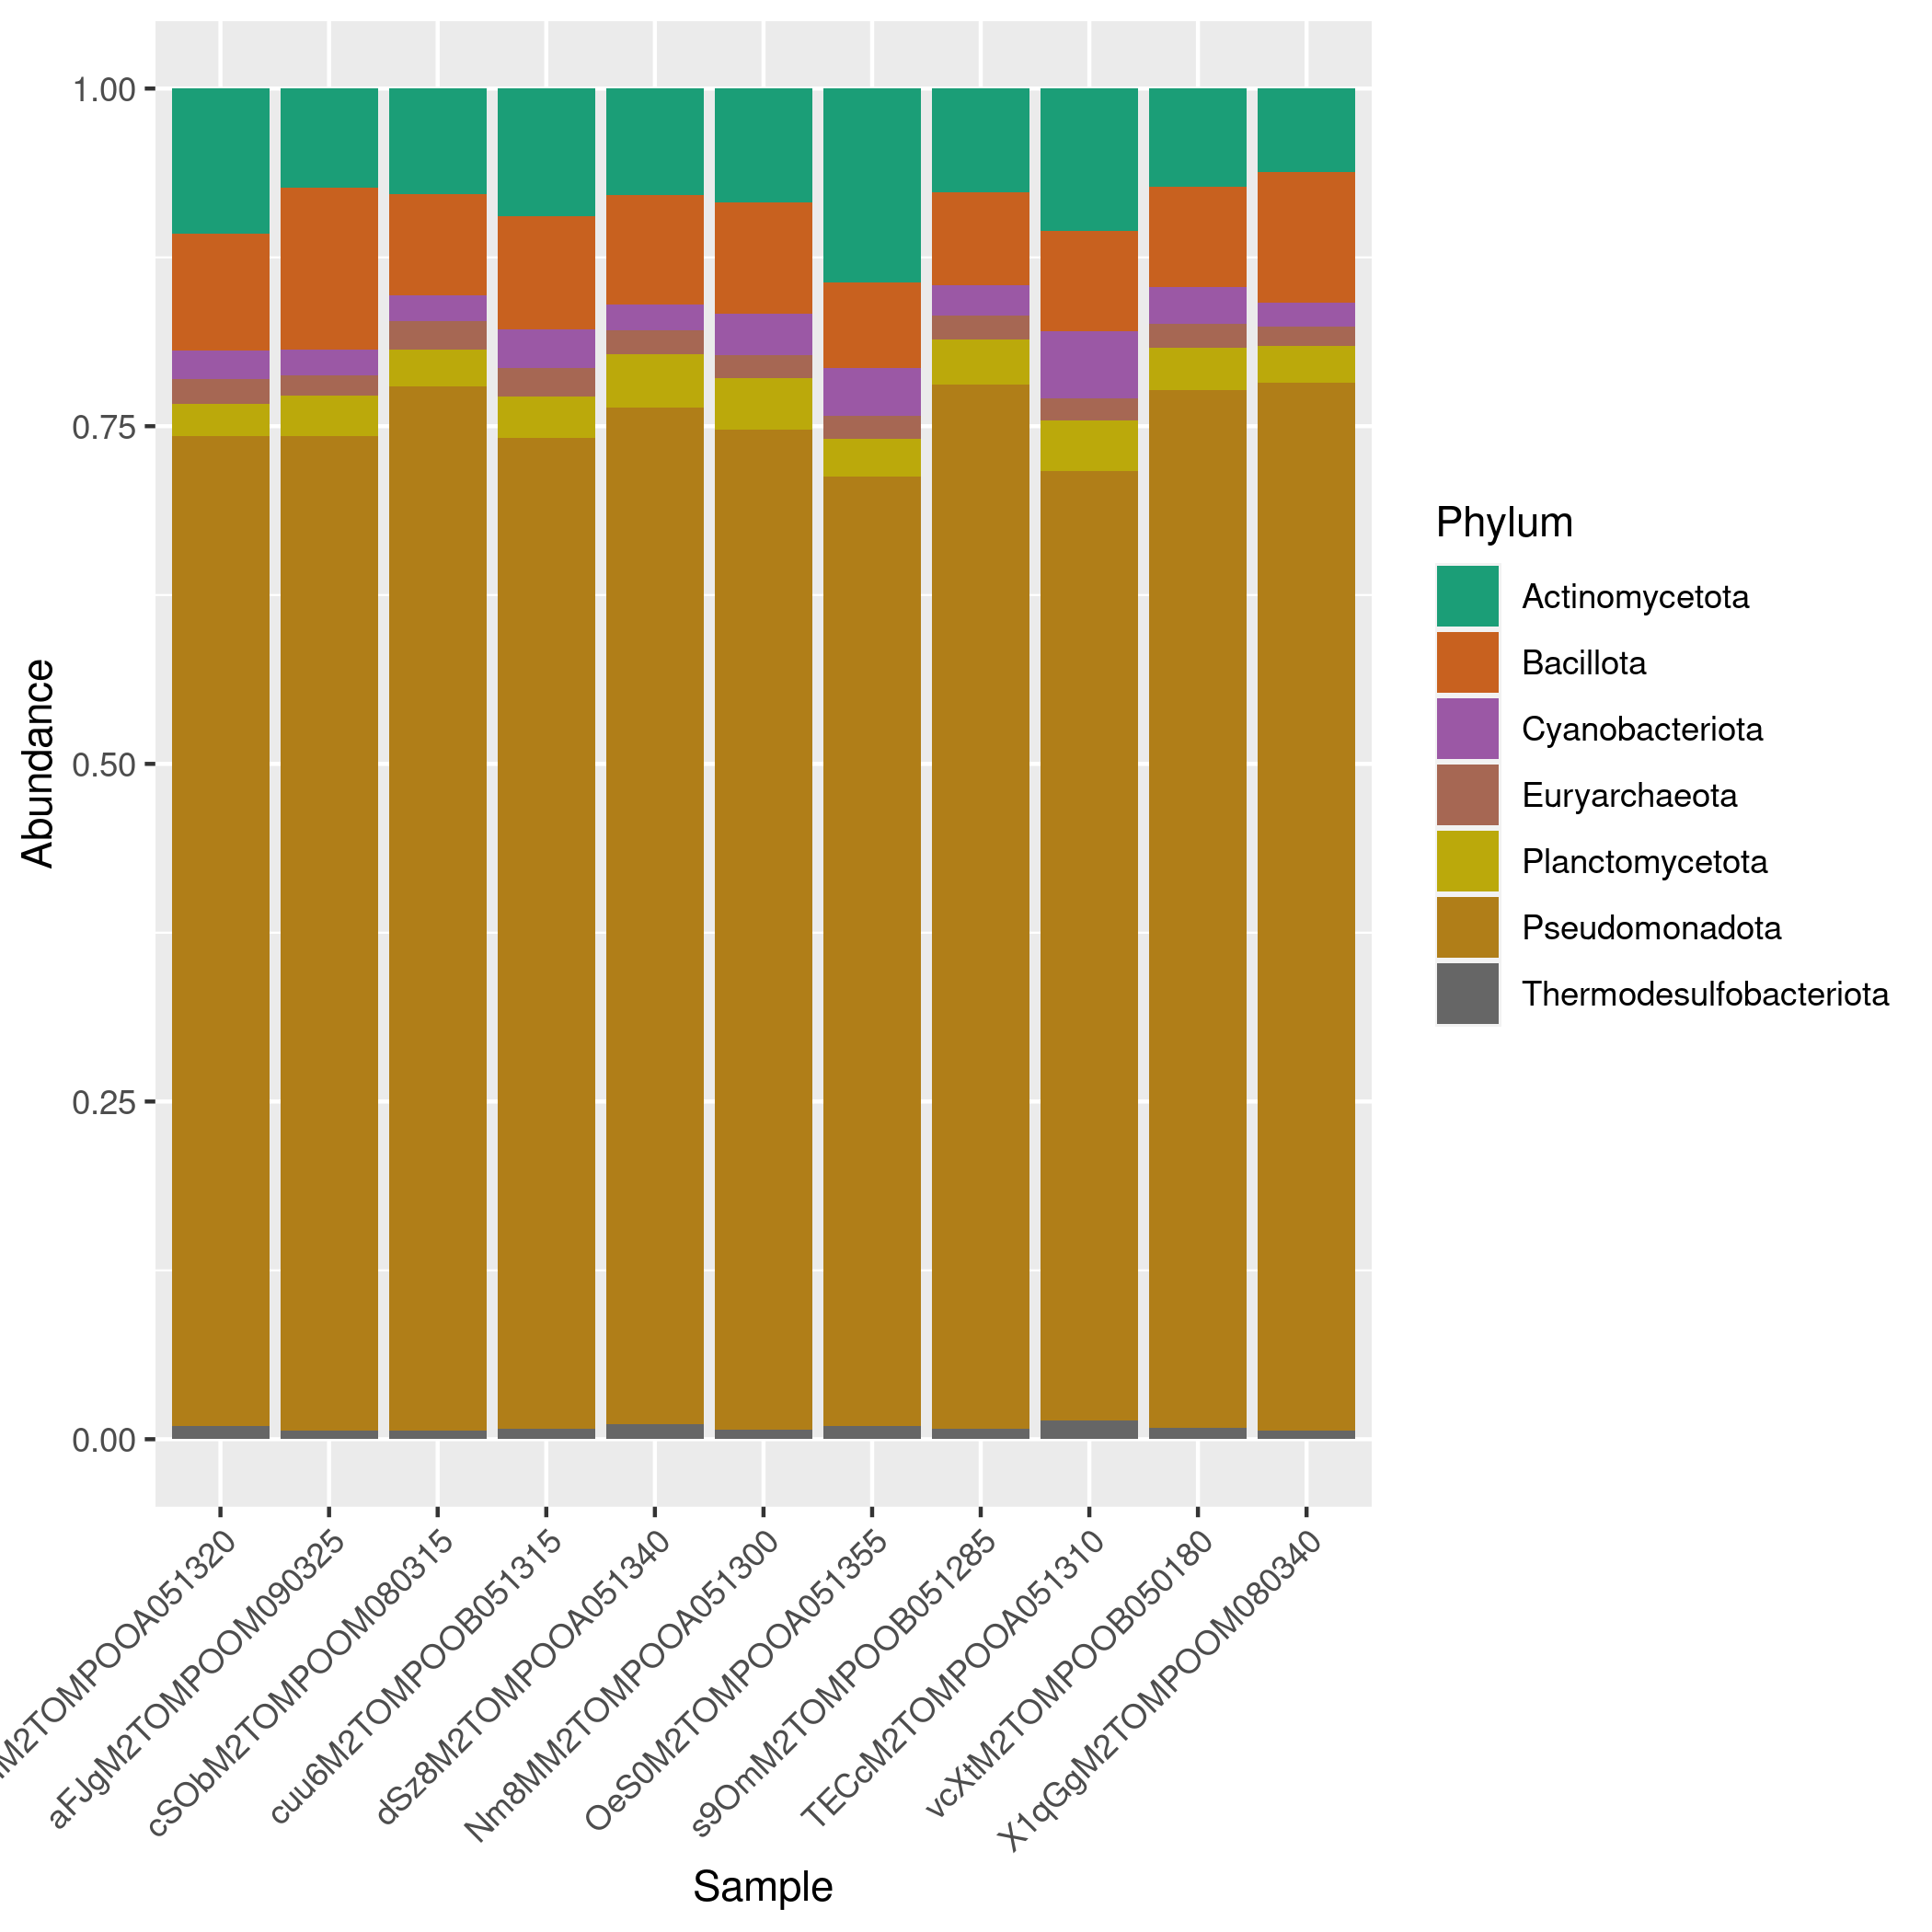
\includegraphics[scale = 0.8]{tomate_aleatorio1_1.csv_relative_abundance_Phylum.png}
\caption{Relative abundance by phyla of keystone OTUs }
\label{fig:tomate_aleatorio1_1.csv_phyla}
\end{figure}
\begin{figure}
\centering
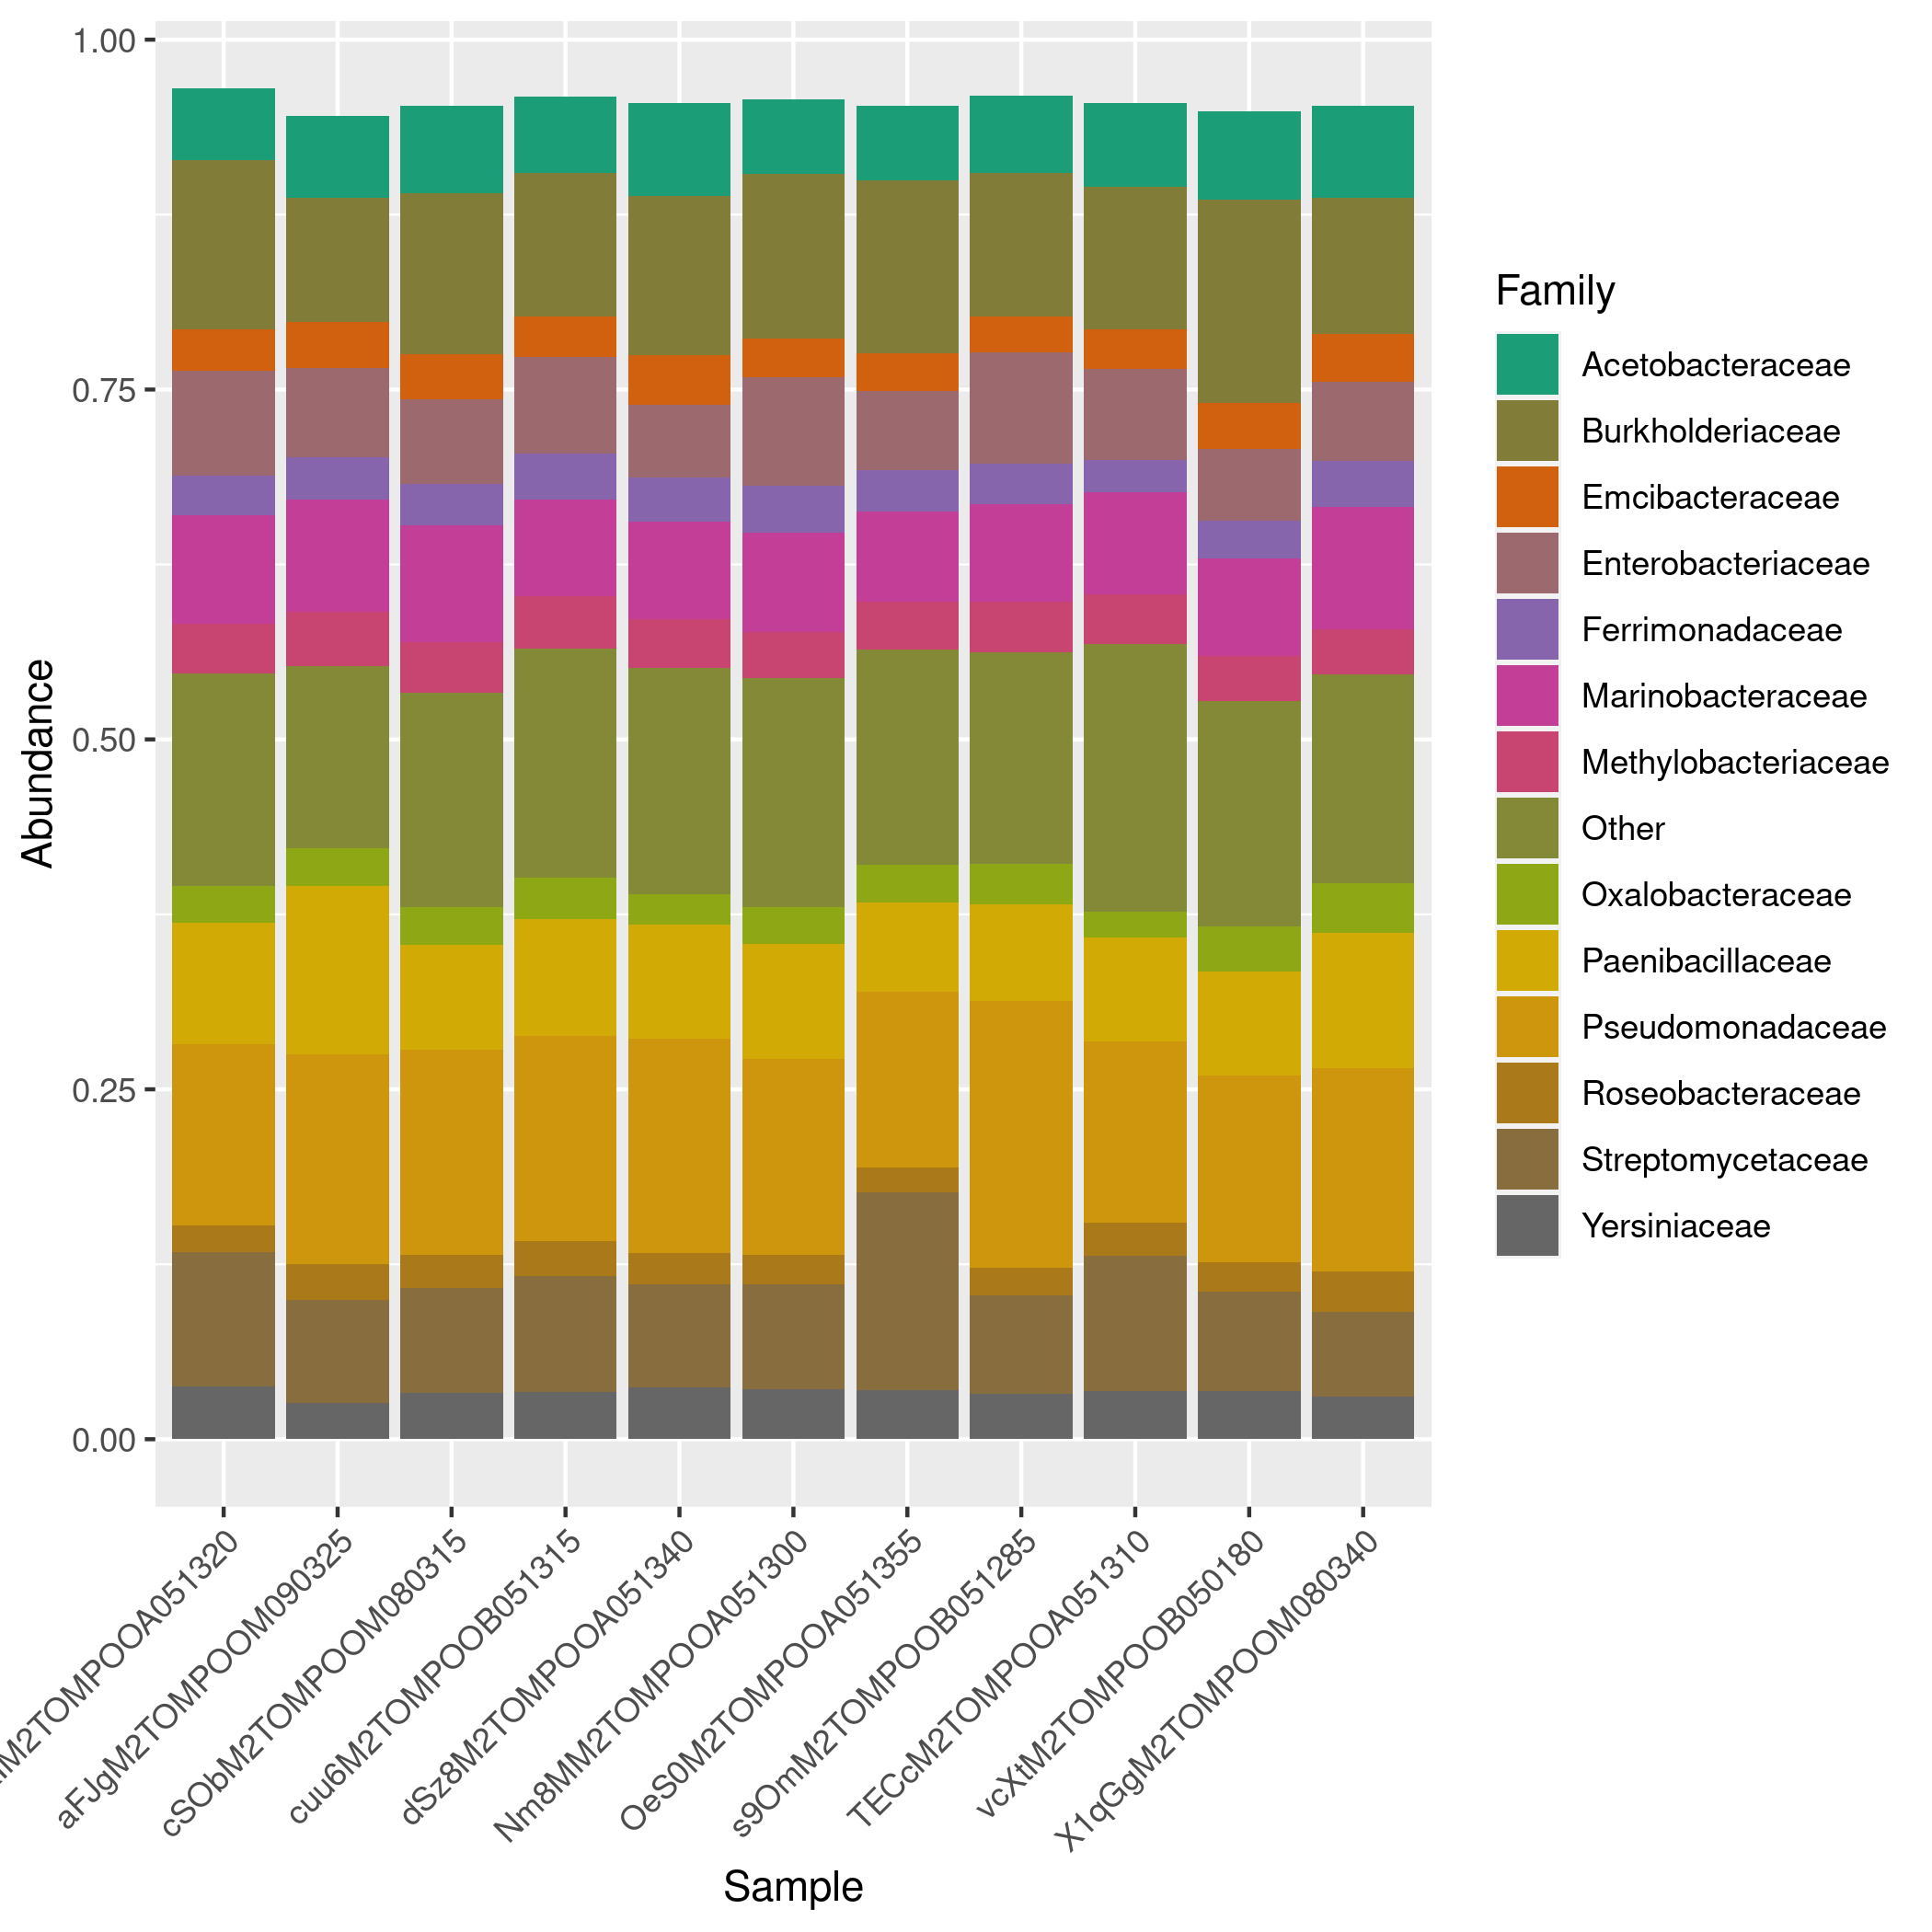
\includegraphics[scale = 0.8]{tomate_aleatorio1_1.csv_relative_abundance_Family.png}
\caption{Relative abundance by families of keystone OTUs }
\label{fig:tomate_aleatorio1_1.csv_family}
\end{figure}
\begin{figure}
\centering
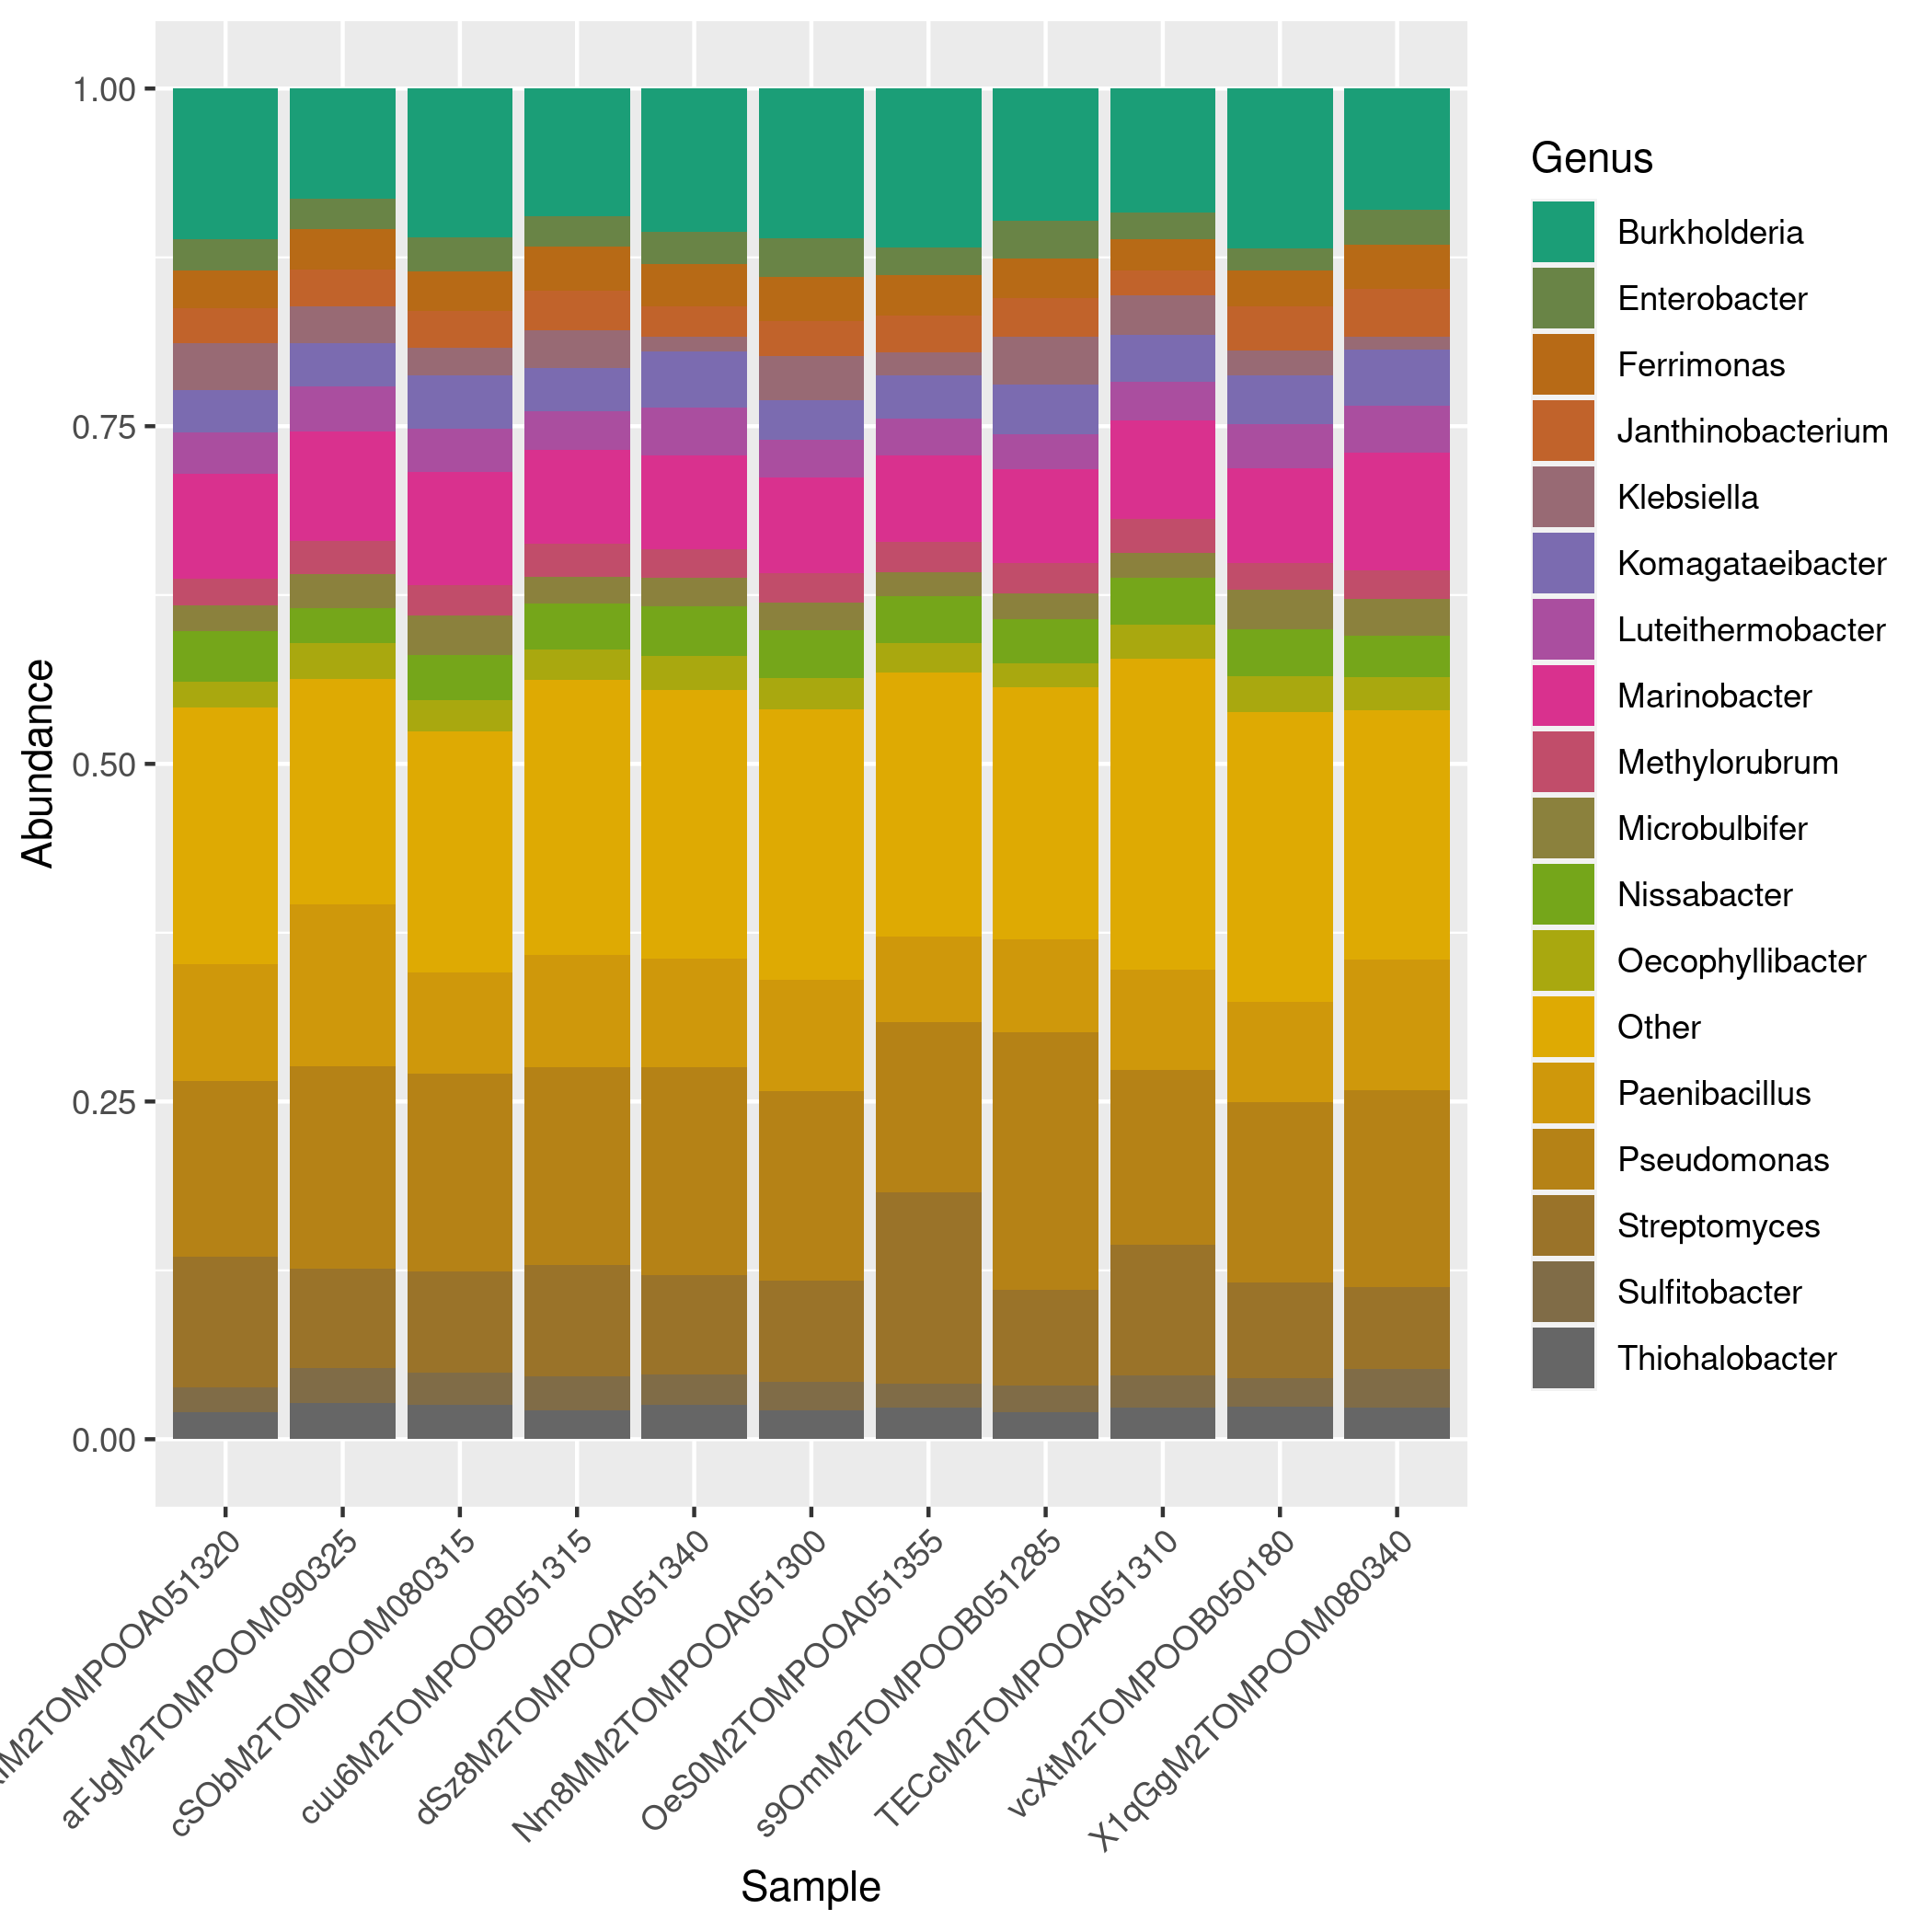
\includegraphics[scale = 0.8]{tomate_aleatorio1_1.csv_relative_abundance_Genus.png}
\caption{Relative abundance by genera of keystone OTUs }
\label{fig:tomate_aleatorio1_1.csv_genus}
\end{figure}
\begin{figure}
   \centering
   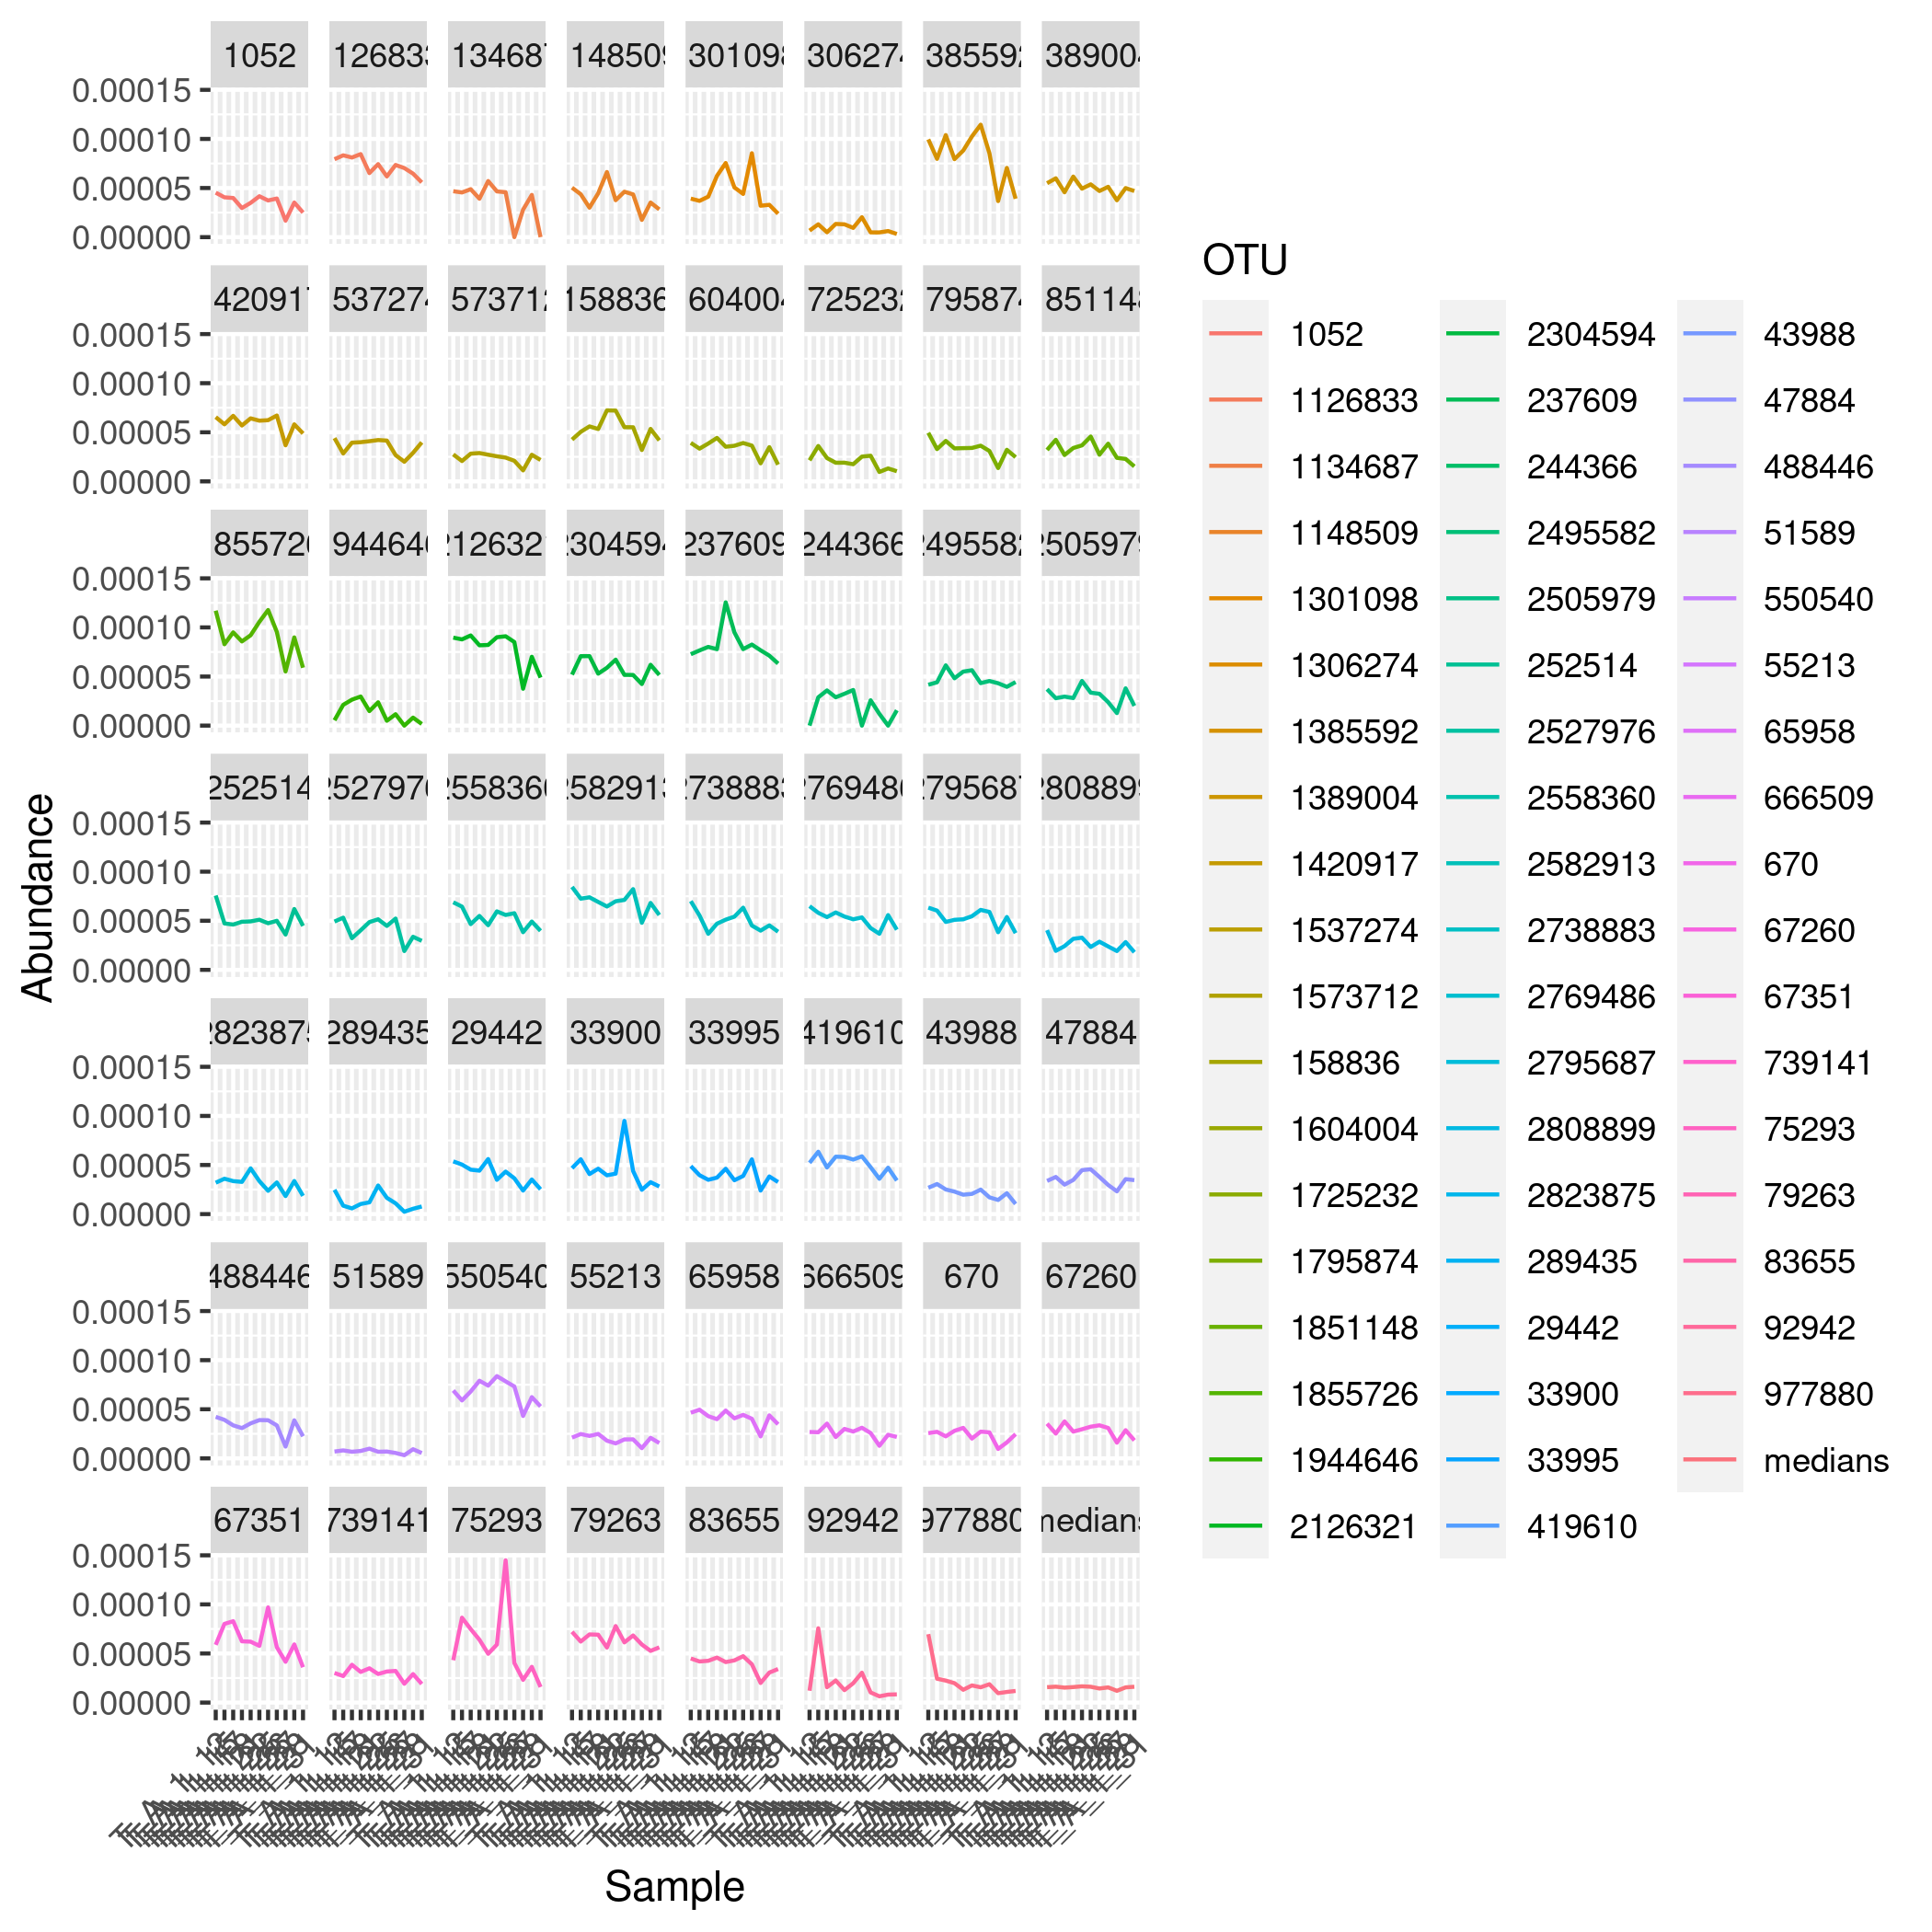
\includegraphics[scale = 0.8]{abundance_tomate_aleatorio1_1.csv_key_otus_medians.png}
   \caption{Plots representing relative abundance of each keystone OTU and one representing the median relative abundance  across samples of rhizosphere of tomate_aleatorio1_1.csv. Most keystone OTUs have relative abundance bigger than the median across all samples.  }
   \label{key_otus_vs_medians_tomate_aleatorio1_1.csv}
\end{figure}
\begin{figure}
 \centering
 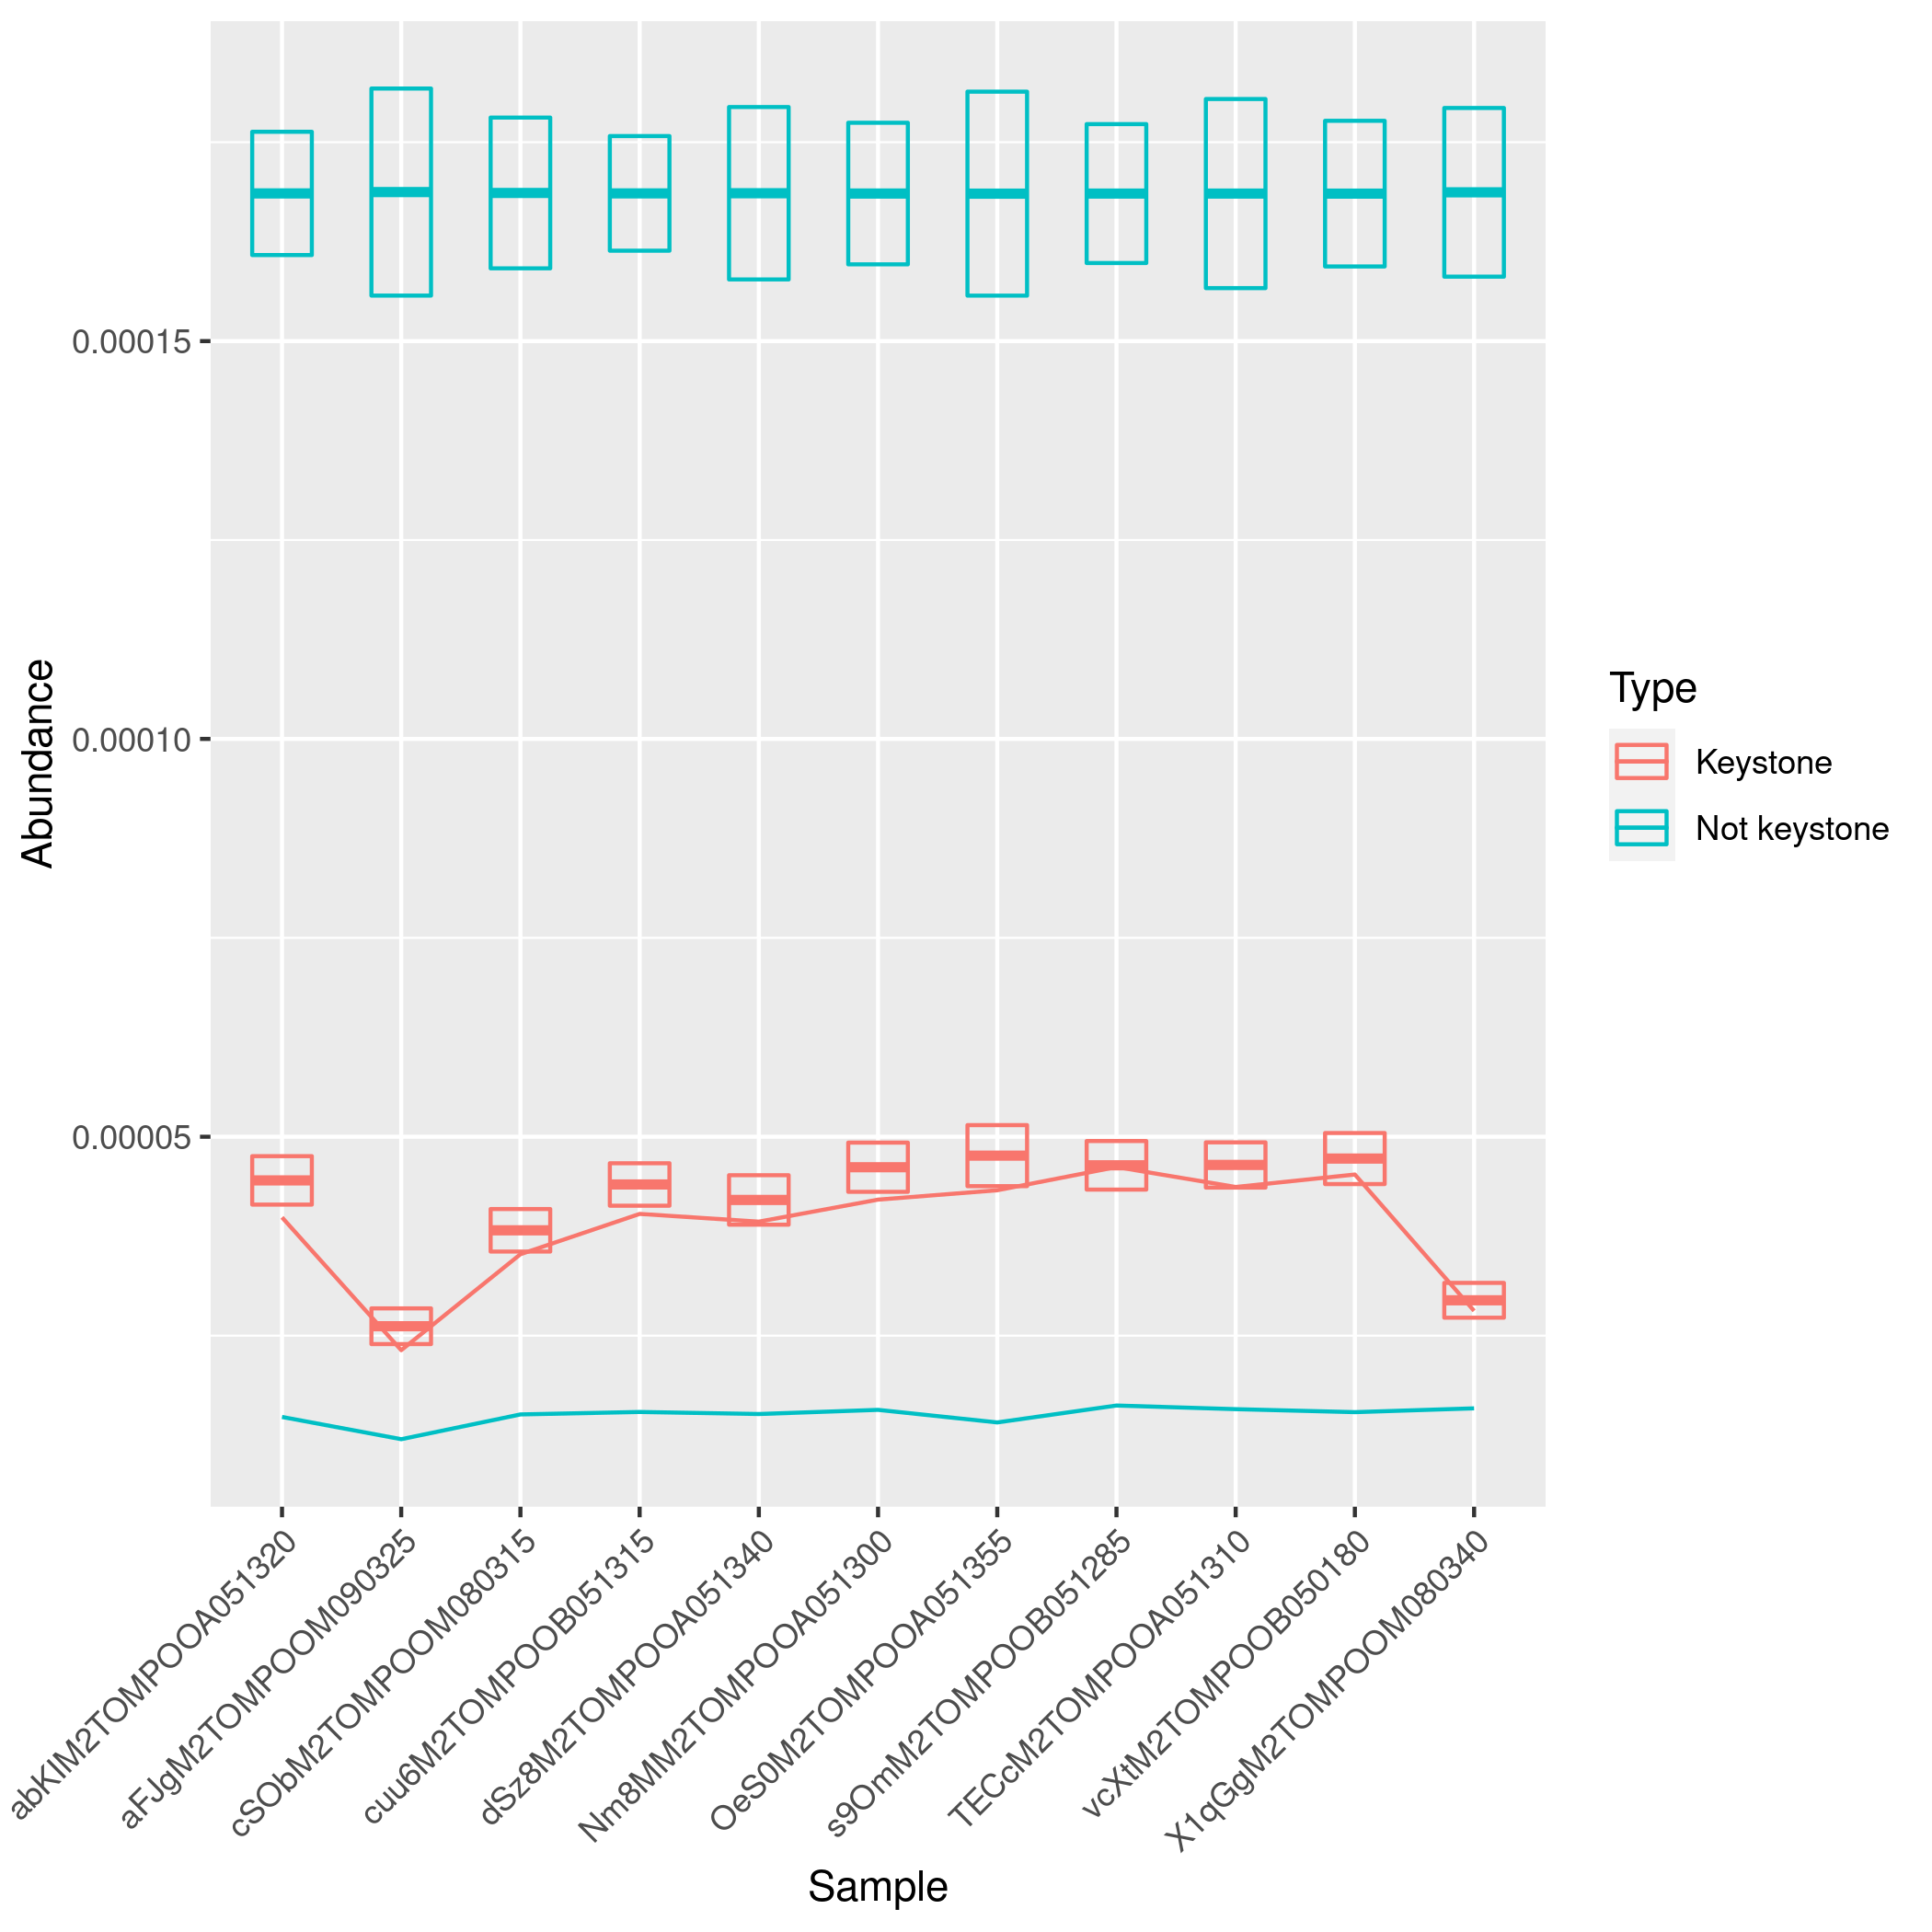
\includegraphics[scale = 0.75]{mean_median_key_vs_not_key_tomate_aleatorio1_1.csv.png}
\caption{Boxes represent mean and standard error in the distribution of corresponding samples. Lines represent the corresponding medians. In these samples of rhizosphere oftomate_aleatorio1_1.csv}
\label{mean_median_tomate_aleatorio1_1.csv}
\end{figure}
\begin{figure}
   \centering
   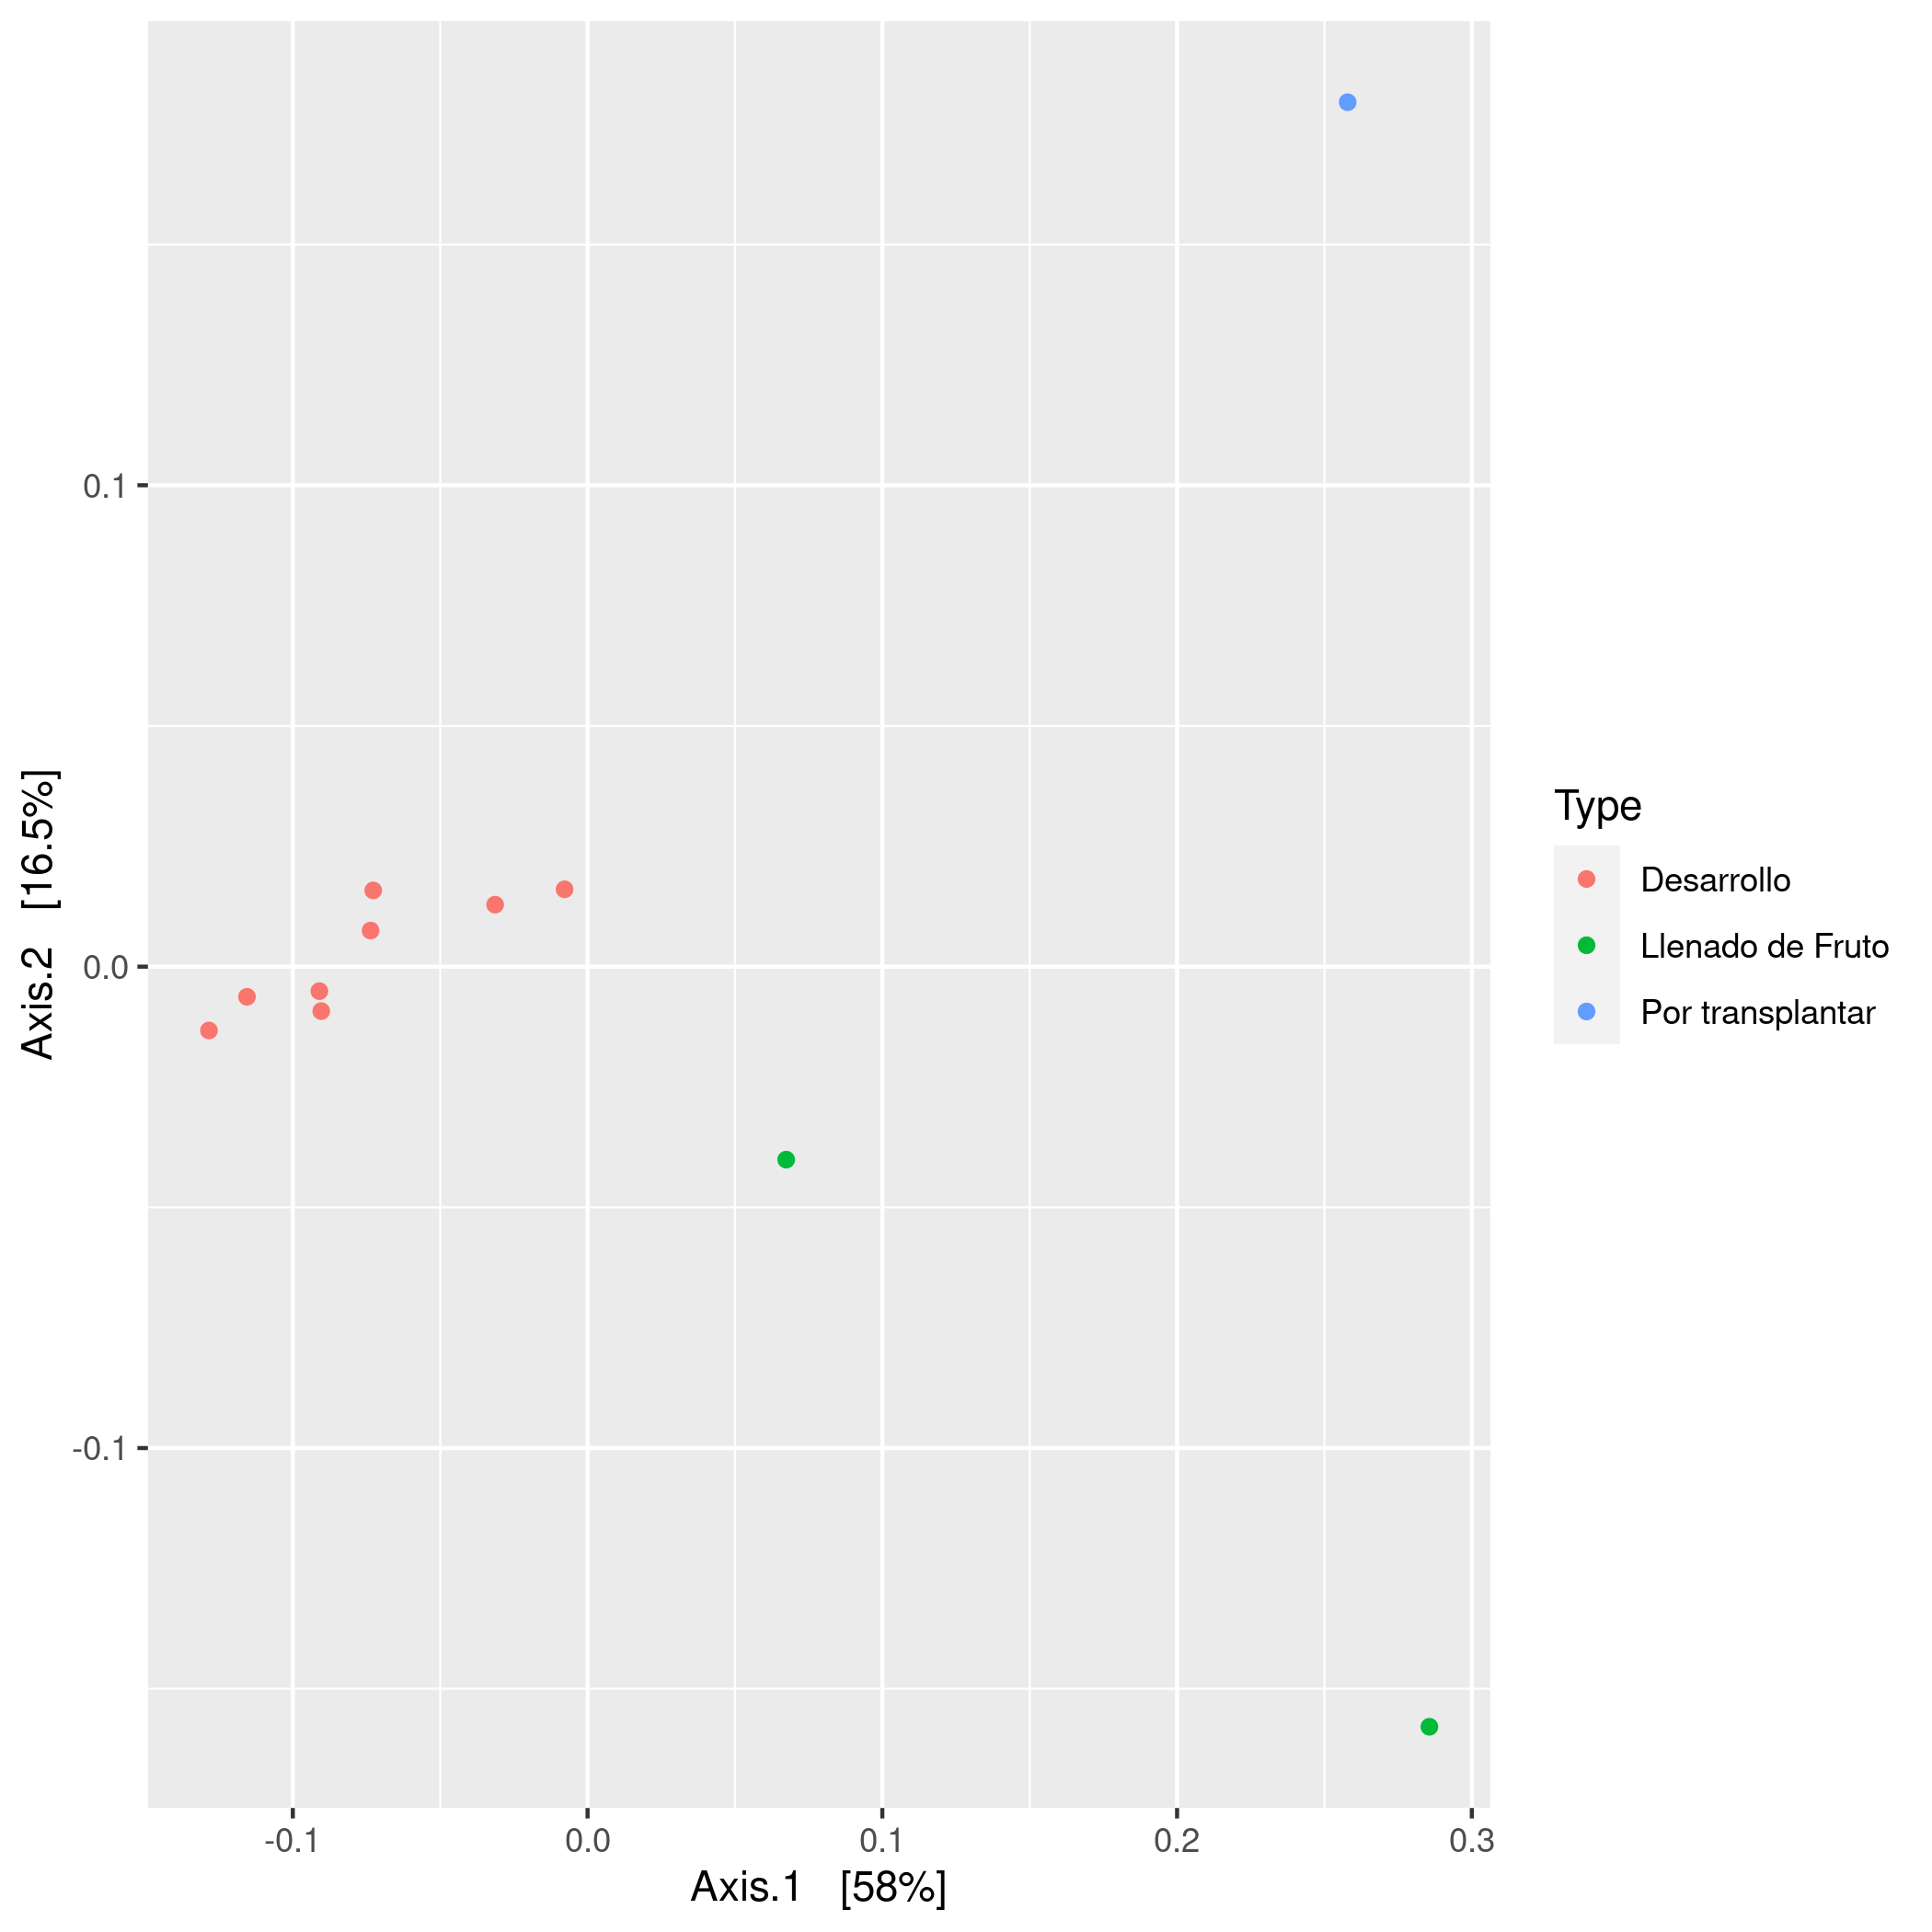
\includegraphics[scale = 0.7]{pcoa_muestras_tomate_aleatorio1_1.csv.png}
 \caption{PCoA analysis with Bray-Curtis distance of rhizosphere samples of tomate_aleatorio1_1.csv.}
 \label{fig:tomate_aleatorio1_1.csv_pcoa}
\end{figure}
\begin{figure}
  \centering
  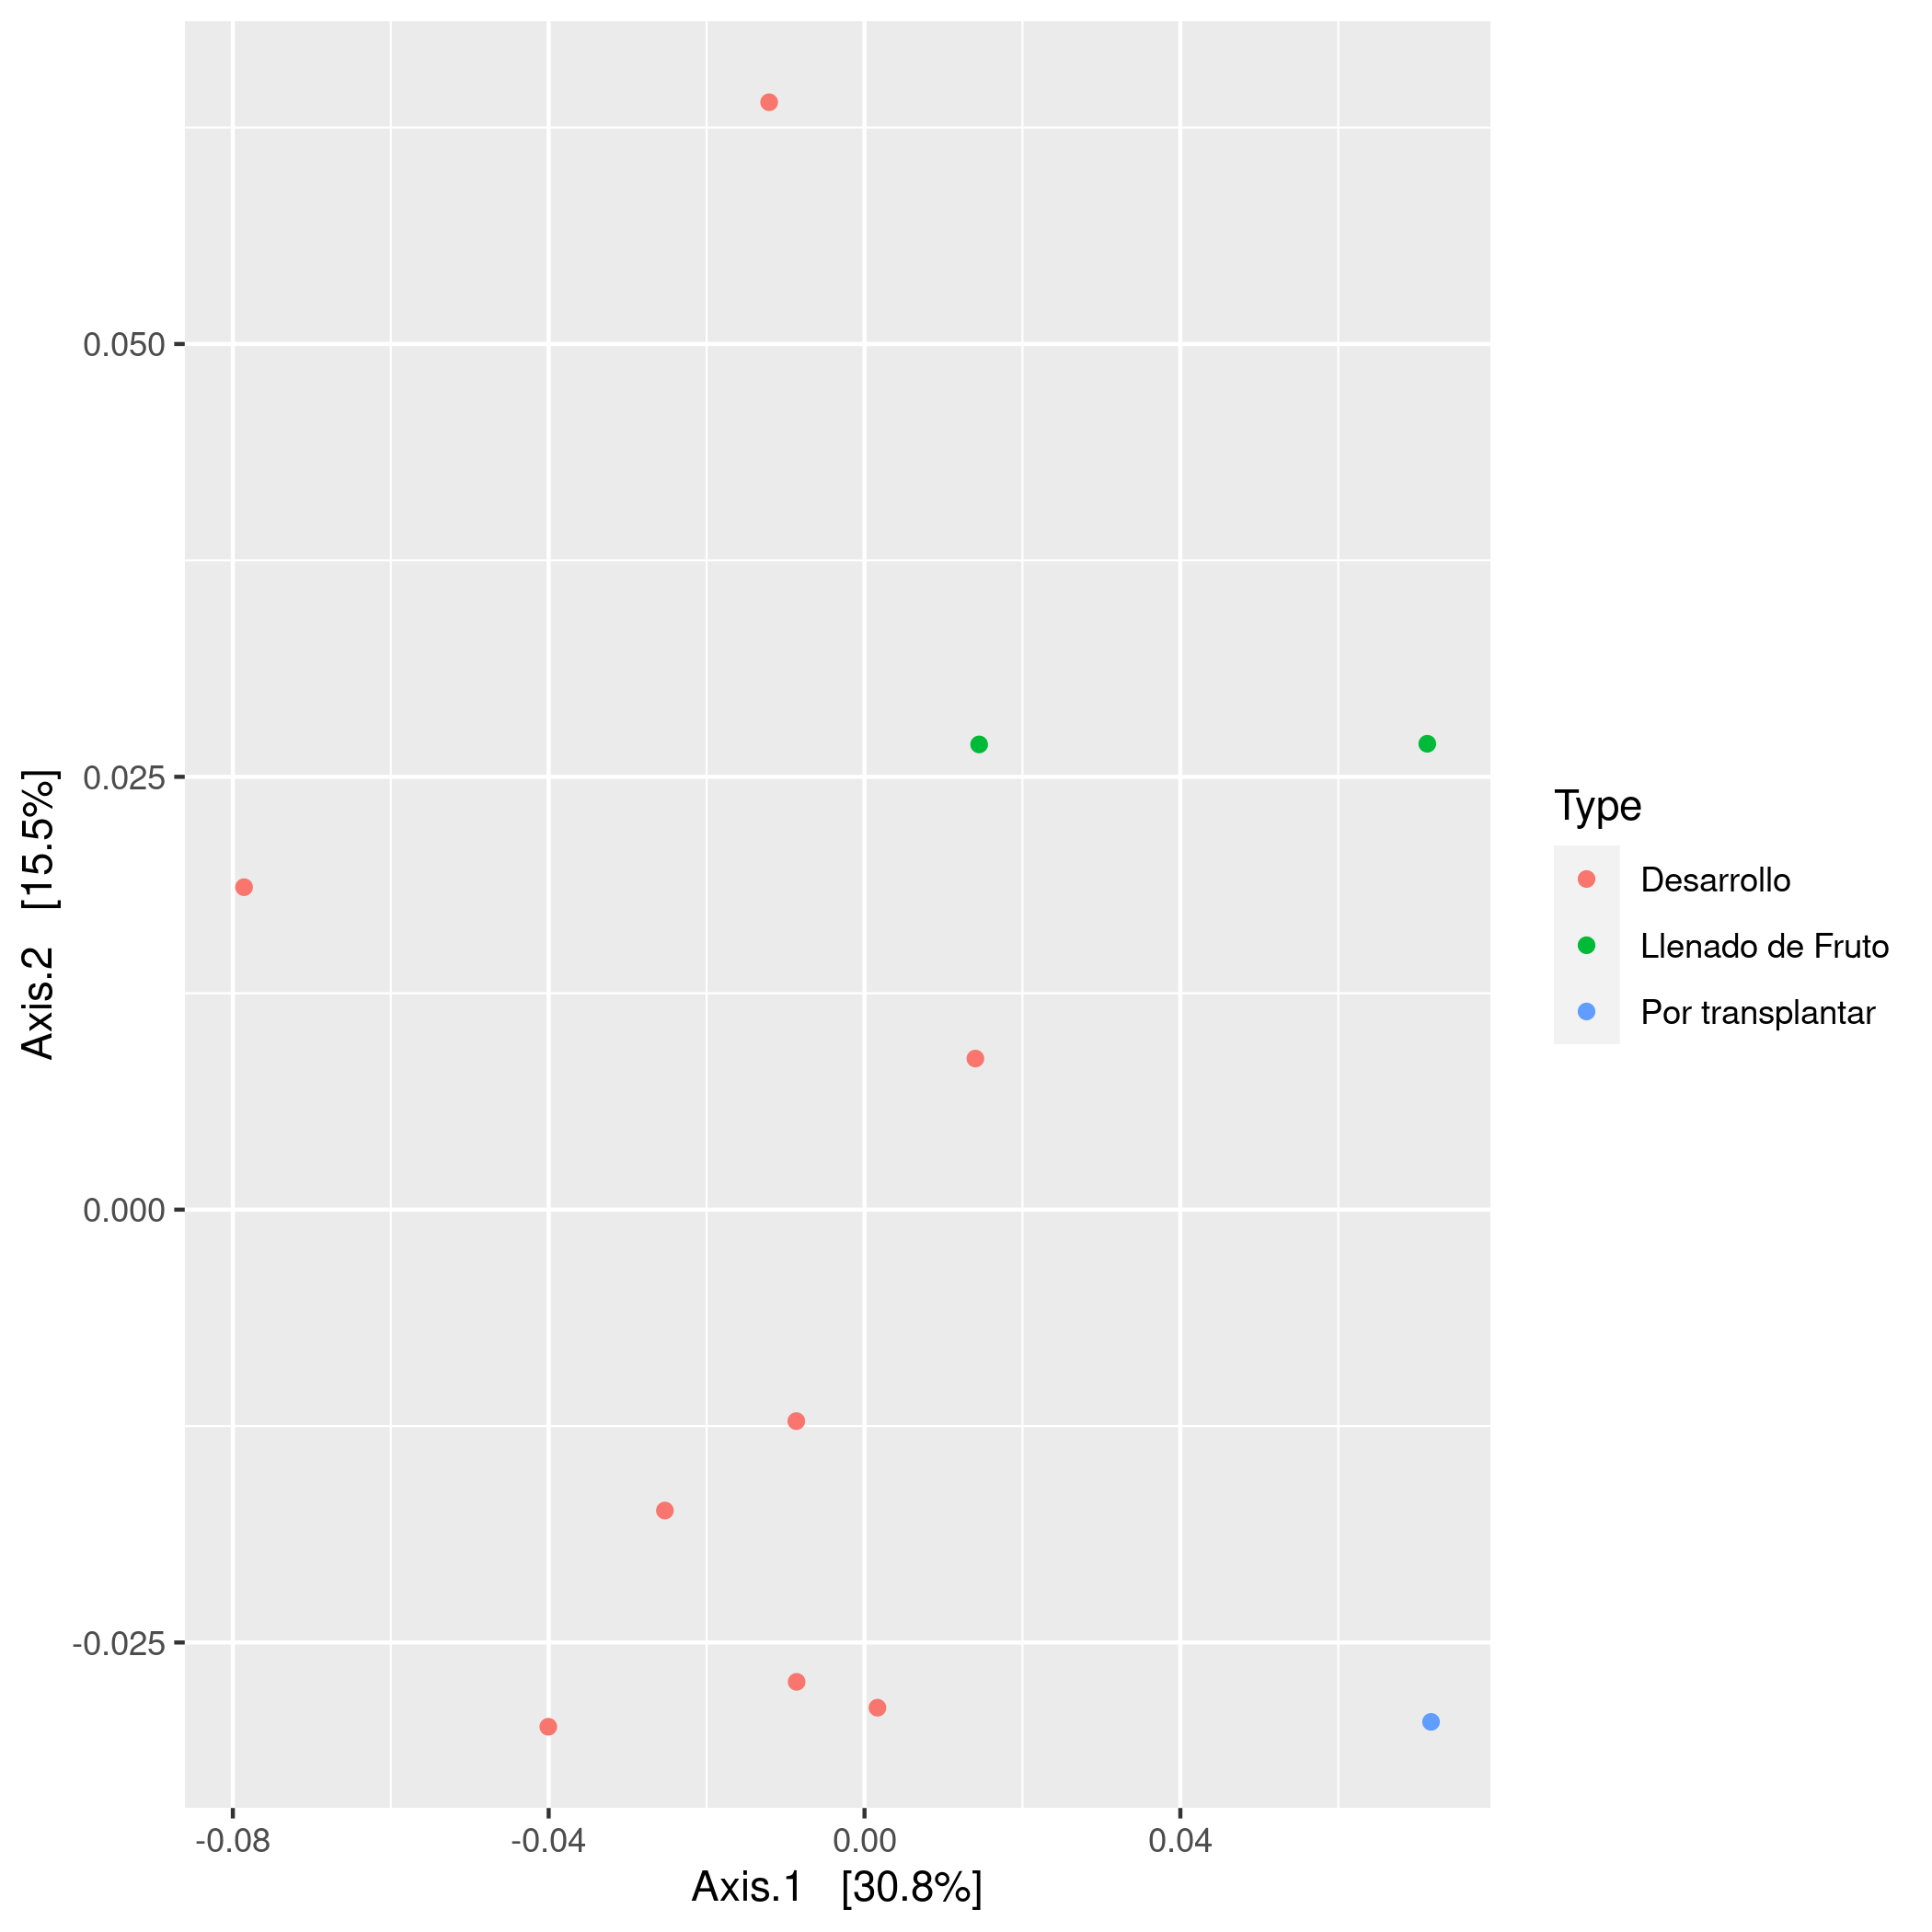
\includegraphics[scale = 0.7]{pcoa_key_otus_tomate_aleatorio1_1.csv.png}
  \caption{PCoA analysis with Bray-Curtis distance of rhizosphere samples of tomate_aleatorio1_1.csv, restricted to keystone OTUs.}
  \label{fig:tomate_aleatorio1_1.csv_pcoa_key_otus}
\end{figure}
